\begin{tiny}(Edg02)\end{tiny}
\begin{figure}[h!t]
 \centering
 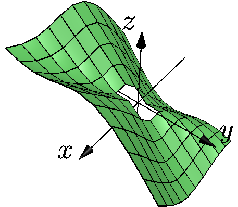
\includegraphics{./Edg02_2.pdf}
 \caption{Exercice \arabic{enumi} . Le graphe d'une fonction. Mais laquelle ?}
 \label{fig:Edg02_2}
\end{figure}
\begin{figure}[h!t]
 \centering
 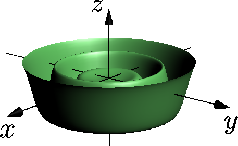
\includegraphics{./Edg02_1.pdf}
 % Edg02_1.pdf: 167x199 pixel, 72dpi, 5.89x7.02 cm, bb=0 0 167 199
 \caption{Exercice \arabic{enumi} . Le graphe d'une fonction. Mais laquelle ?}
 \label{fig:Edg02_1}
\end{figure}
\begin{figure}[h!t]
 \centering
 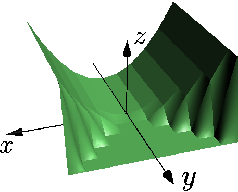
\includegraphics{./Edg02_4.pdf}
 \caption{Exercice \arabic{enumi} . Le graphe d'une fonction. Mais laquelle ?}
 \label{fig:Edg02_4}
\end{figure}
\begin{figure}[h!t]
 \centering
 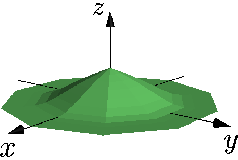
\includegraphics{./Edg02_3.pdf}
 \caption{Exercice \arabic{enumi} . Le graphe d'une fonction. Mais laquelle ?}
 \label{fig:Edg02_3}
\end{figure}

\'Etudier la continuit{\'e}, l'existence et la continuit{\'e} des d{\'e}riv{\'e}es partielles pour les fonctions $f$ suivantes
\begin{align*}
&\left\{
\begin{aligned}
(x^{2}+y^{2})\sin \frac{1}{x^{2}+y^{2}} & \text{ si } & (x,y)\neq (0,0) \\
0 & \text{ si } & (x,y)=(0,0)
\end{aligned}
\right.  \\
&\left\{
\begin{aligned}
\frac{x^{3}-y^{3}}{x^{2}+y^{2}} & \text{ si } & (x,y)\neq (0,0) \\
0 & \text{ si } & (x,y)=(0,0)
\end{aligned}
\right.  \\
&\left\{
\begin{aligned}
e^{\frac{1}{x^{2}+y^{2}-1}} & \text{ si } & x^{2}+y^{2}<1 \\
0 & \text{ si } & x^{2}+y^{2}\geq 1
\end{aligned}
\right.  \\
&\left\{
\begin{aligned}
x^{2} & \text{ si } & \left| x\right| >y \\
0 & \text{ si } & \left| x\right| \leq y
\end{aligned}
\right.
\end{align*}